\documentclass{article}
\usepackage[utf8]{inputenc}
\usepackage{fancyhdr}
\usepackage{graphicx}
\usepackage{float}
\usepackage{geometry}
\usepackage[font=small,labelfont=bf]{caption}
\usepackage{caption}
\captionsetup[figure]{font=small}
\usepackage[justification=centering]{caption}
\usepackage{courier}

% ---- Commands ------- %
\newcommand{\documentNumber}[1]{
    \LARGE  \textbf{ PUSS21420{#4} } \\
    \medskip
}
\newcommand{\documentVersion}[1]{
    v. {#1}

    \medskip
}
\newcommand{\documentTitle}[1]{
    \centerline{\rule{12cm}{0.4pt}}
    \bigskip \bigskip
    \LARGE \textbf{TimeMate} \\
    \bigskip
    \LARGE {#1} \\
    \bigskip \bigskip
    \centerline{\rule{13cm}{0.4pt}}
}
\newcommand{\documentGroup}[1]{
    \bigskip \bigskip
    \LARGE Group {#1} \\
    \bigskip
}
\newcommand{\documentResponsible}[1]{
    \LARGE Responsible: {#1} \\
    \medskip
}
\newcommand{\documentAuthors}[1]{
    \LARGE Authors: {#1} \\
    \medskip    
}
\newcommand{\documentDate}[1]{
    \date {#1} 
}

\graphicspath{{./images/}} % Defines a path to file images
\renewcommand{\arraystretch}{1.7}  % Vertical padding for tables


% --- Header & Footer ---- %
\pagestyle{fancy}
\lhead{\leftmark}
\rhead{}
\rfoot{\thepage}
\cfoot{}
\lfoot{}


% ------------------------------------------------ #

% ----- FILL THIS ----- %
\title {
    % Must be 2 digits
    \documentNumber {01}    
    
    % BASELINE.VERSION
    \documentVersion {0.3}
    
    % Full name - SHORTNAME
    \documentTitle {Software Top Level Design Document}
    \documentGroup {2}
    
    % Options: - Project Management Group
    %          - System Architecture Group
    %          - Developer Group
    %          - Test Group
    \documentResponsible {System Group}
    \documentAuthors {Developer Group}
    
    % Format: YYYY-MM-DD
    \documentDate {2021-02-18}
}

\begin{document}

\maketitle
\thispagestyle{empty}

\newpage

\tableofcontents

\newpage

%---------Document begins here-----------

% FILL IN CORRECT VERSION HISTORY!
% Not sure? Refer to SDP how it works or ask someone!
\section{Document History}
\begin{tabular}{ l | l | l | l }
    Version & Date & Responsible & Description \\
    \hline
    0.1 & 2021-02-11 & UG & Document created. \\
    \hline
    0.2 & 2021-02-17 & UG & Ready for informal review. \\
    \hline
    0.3 & 2021-02-18 & UG & Corrected grammar and more after informal review \\
\end{tabular}

\section{Introduction}
This document describes the design of TimeMate. The system is a further development of the system BaseBlockSystem. TimeMate hosts various functions related to the creating of time reports, getting a view of reported time and more.

\section{Reference Documents}
\begin{enumerate}
    \item Software Requirements Specification: TimeMate, v. 1.1, Doc. number: PUSS214201
    \item Software Top Level Design Document: BaseBlockSystem, v 1.0, Doc. number: PUSS12004
\end{enumerate}

\section{Terminology}
\begin{itemize}
\item \textbf{Java Server Page (JSP):} Server-side technology that enables the creation of dynamic views.
\item \textbf{Servlets:} Java programs that run on the server side.
\item \textbf{Java Beans:} A Java class that only contains set/get methods with private attributes. Moreover, a Java Bean must implement the Serializable interface.
\end{itemize}

\section{Overview}
This system is developed using Apache Tomcat, wherein the controllers (Java Servlets) manipulates and sends data to the views (JavaServer Pages).

\subsection{Java Server Pages}
Below are the pages used for TimeMate and what their functions are.

\subsubsection{login.jsp}
This view is shown when a user that is not logged in tries to access the system. This is the only page in the TimeMate system a user can get access to without having an account. The page consists of two fields,  one for username and one for password, as well as an option to request a new password in case the user has forgotten their password.  If the user chooses to reset their password, a pop up is shown where the user can enter their e-mail which the new password will be sent to.

\subsubsection{index.jsp}
This view is shown when a user has logged in. From here,  the user can access the menu which is dynamically updated depending on what group the user belong to. The index page contains an overview of TimeMate.

\subsubsection{newreport.jsp}
This view shows an empty time report. The user can fill in the time report and submit it.

\subsubsection{editreport.jsp}
This view is used by users that want to edit their previously reported time reports. When being here, the user can select a submitted report to edit.

\subsubsection{summaryreport.jsp}
This view represents a summary of a user's previously reported time reports. The user can select a time report to show detailed information about it.

\subsubsection{signreport.jsp}
This view is used by the project leaders for signing and unsigning time reports.

\subsubsection{usermanagement.jsp}
This view shows the user management page. The view is used by the administrator and the project leaders. The view is used for assigning roles to project members.

\subsubsection{administration.jsp}
This view shows the administration page. Only the administrator has access to this view. The view is used for administration purposes such as adding and removing project members. 

\subsubsection{changepassword.jsp}
This view is used by all users to change their password. The page contains three fields, one for the user's current password, and two for the new password (in order to confirm it).

\subsection{Java Beans}
The files below are the Java Beans that are used to send information from the server to the client view. When created, beans are stored in the current session and discarded when the session ends.

\subsubsection{UserBean}
This class contains user information required to execute queries and updates related to the logged in user.

\subsubsection{TimeReportBean}
This class contains a list of users and their time reports which is required to render the report.jsp view.

\subsubsection{TimeReportManagementBean}
This class contains a list of signed time reports which is required to render signReport.jsp.

\subsubsection{UserManagementBean}
This class contains a list of users (excluding project leaders) and their roles which is required to render the userManagement.jsp view.

\subsection{Servlets}
The servlets below are the controllers for the system.

\subsubsection{LoginServlet}
Communication link between the view login.jsp and the bean UserBean.

\subsubsection{PasswordChangerServlet}
Servlet used when a user changes their password.

\subsubsection{TimeReportServlet}
Communication link between the views viewReport.jsp, newReport.jsp and summaryReport.jsp and the bean ReportBean.

\subsubsection{TimeReportManagementServlet}
Communication link between the views editReport.jsp and signReport.jsp and the bean TimeReportManagementBean

\subsubsection{UserManagementServlet}
Communication link between the view userManagement.jsp and the bean UserManagementBean.


\subsection{Other classes}
The classes below are never accessed by the user in any way, but are instead helper classes to the servlets.

\subsubsection{MailHandler}
Class used to send e-mails to users upon account creation and password changes.

\subsubsection{PasswordHandler}
Class used to encrypt and generate new passwords.

\subsubsection{Database}
Class used to establish connection between Tomcat and the database as well as executing all queries to the database.

\section{Database}
In this project, there is one database that consists of the nine relations shown in Figure 1. Every relation has one primary key each, which are the following: \emph{userName} and \emph{reportID}.

\begin{figure}[H]
     \centering
     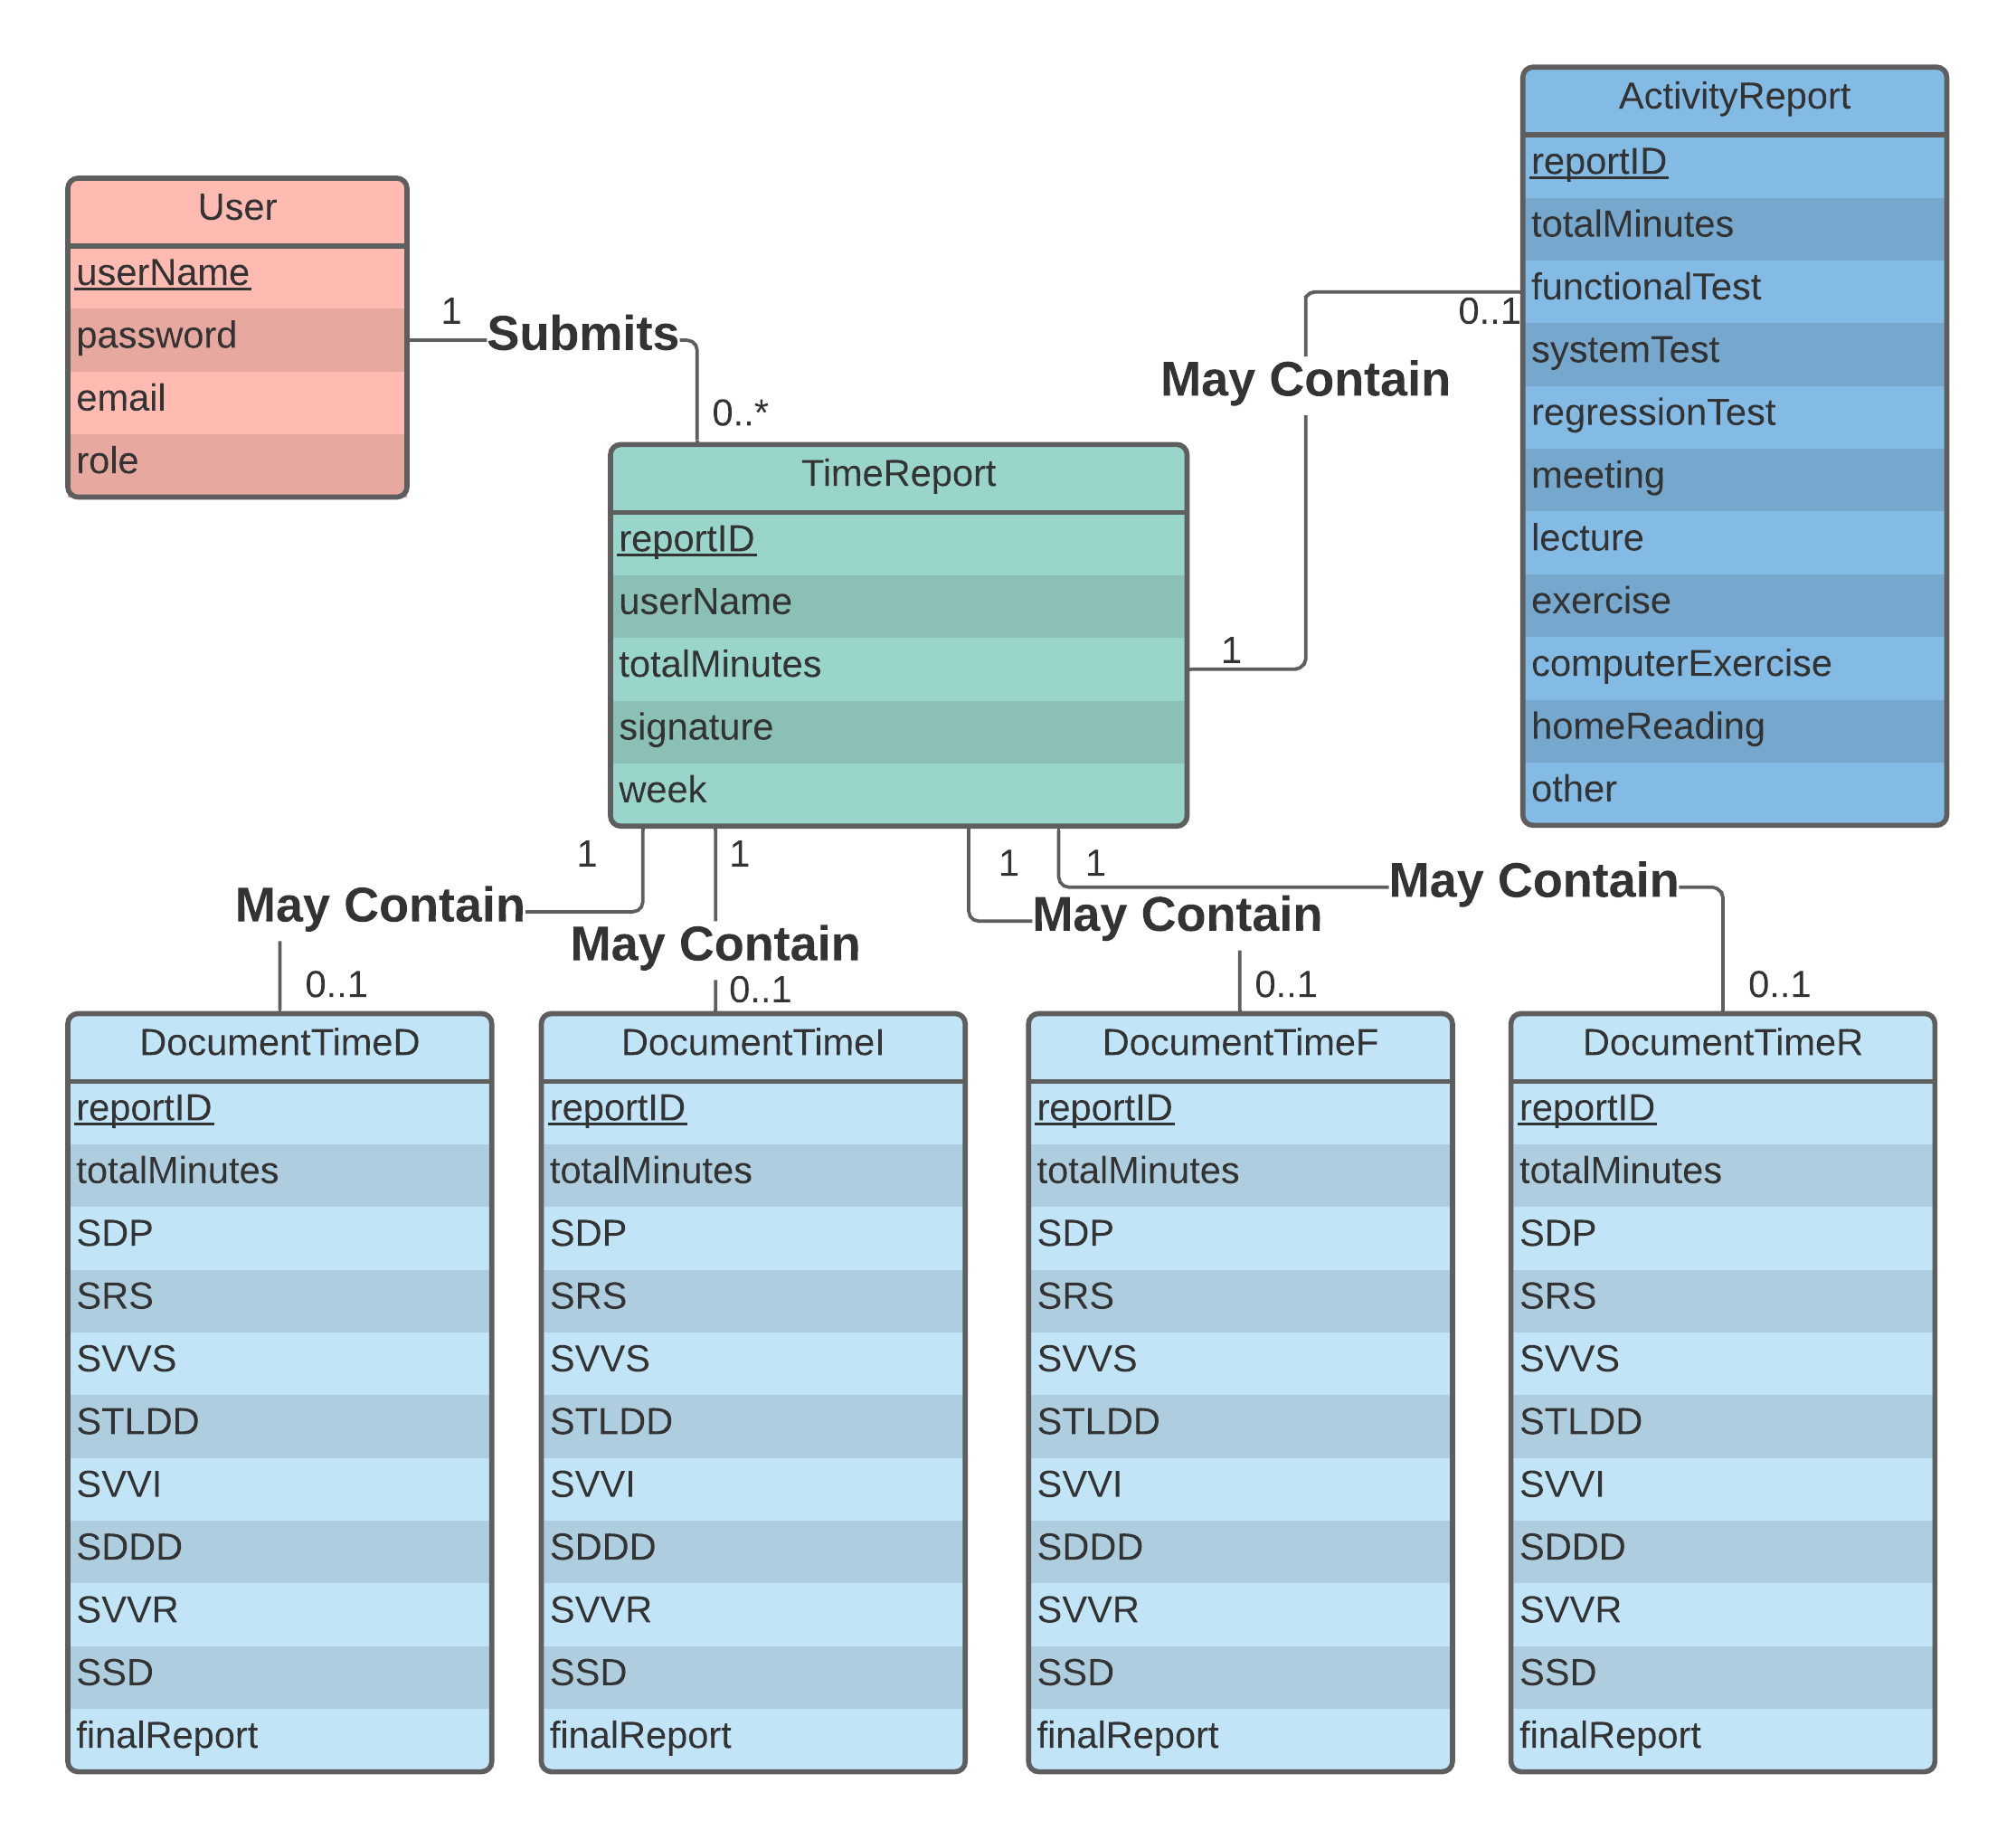
\includegraphics[width=13cm]{images/PUSPERdiagramVers3_2.png}
     \renewcommand\figurename{Figure}
     \caption{The database consists of the following relations: \emph{User},  \emph{TimeReport}, \emph{ActivityReport} and \emph{DocumentTimeD/I/F/R}.}
     \label{fig:my_label}
 \end{figure}

\subsection{User Relation}
The User relation contains all registered users together with user specific information such as password, email and information about whether a user belongs to a project group or not. A user belonging to a group may be assigned a role under the role attribute. The userName attribute is used as the primary key, making every username unique. The appearance of the table can be viewed in Figure 2.

\begin{figure}[H]
     \centering
     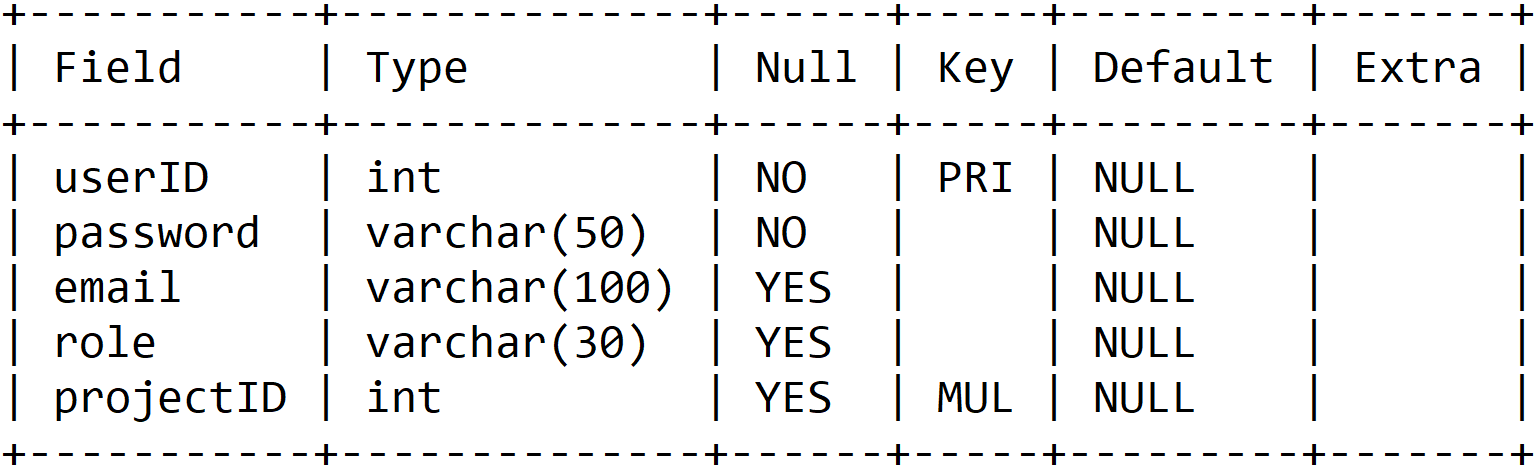
\includegraphics[width=11cm]{images/SQL_tables/user.png}
     \renewcommand\figurename{Figure}
     \caption{A view of the User relation and its attributes.}
     \label{fig:my_label}
 \end{figure}

A User table can be created using the following MySQL command:
\newline

\small
\texttt{
\noindent mysql> CREATE TABLE User (\newline
\indent\indent\indent -> userName Integer NOT NULL,\newline
\indent\indent\indent -> password varChar(50) NOT NULL,\newline
\indent\indent\indent -> email varChar(100),\newline
\indent\indent\indent -> role varChar(30),\newline
\indent\indent\indent -> projectID Integer,\newline
\indent\indent\indent -> PRIMARY KEY(userName)\newline
\indent\indent\indent -> ON UPDATE CASCADE ON DELETE SET NULL\newline
\indent\indent\indent -> );\newline
}
\normalsize
\newpage
\subsection{TimeReport Relation}
The time report to be filled out by each individual user on a weekly basis contains 55 columns, aiming to help the user specify the time spent on various activities. Four sections - \emph{D (Development)}, \emph{I (Informal review)}, \emph{F (Formal review)}, \emph{R (Rework, improvement or correction)}. However, there may be weeks where no time is spent on, e.g.,  formal reviews. In that case, a large number of columns would be wasted, as there will be no meaningful data added to the columns related to that section of the time report.  The appearance of the table can be viewed in Figure 3.

\begin{figure}[H]
     \centering
     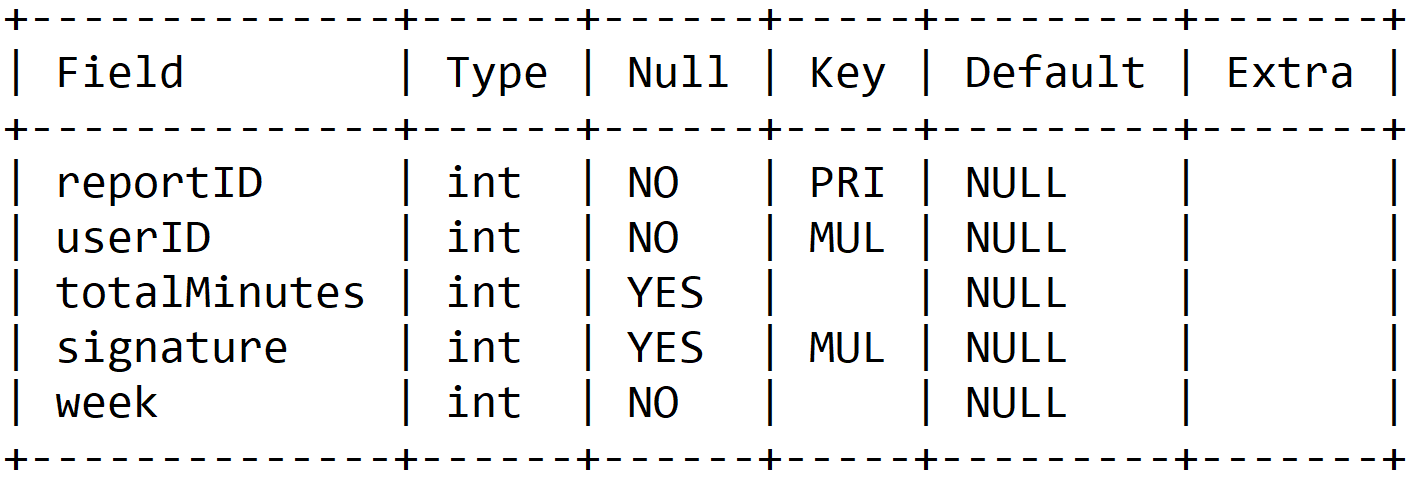
\includegraphics[width=11cm]{images/SQL_tables/timereport.png}
     \renewcommand\figurename{Figure}
     \caption{A view of the TimeReport relation and its attributes.}
     \label{fig:my_label}
 \end{figure}
\newline

A TimeReport table can be created using the following MySQL command:
\newline

\small
\texttt{
\noindent mysql> CREATE TABLE TimeReport (\newline
\indent \indent \indent -> reportID Integer NOT NULL,\newline
\indent \indent \indent -> userName Integer NOT NULL,\newline
\indent \indent \indent -> totalMinutes Integer,\newline
\indent \indent \indent -> signature Integer,\newline
\indent \indent \indent -> week Integer NOT NULL,\newline
\indent \indent \indent -> PRIMARY KEY(reportID),\newline
\indent \indent \indent -> FOREIGN KEY(userName) REFERENCES User(userName)\newline
\indent \indent \indent -> ON UPDATE CASCADE ON DELETE CASCADE,\newline
\indent \indent \indent -> FOREIGN KEY(signature) REFERENCES User(userName)\newline
\indent \indent \indent -> ON UPDATE CASCADE ON DELETE SET NULL\newline
\indent \indent \indent -> );
}
\normalsize
\newline

To avoid data redundancy, the time reports are being separated into several different relations. The reason for this is the fact that every single submitted time report is going to be represented in TimeReports.

\subsection{ActivityReport Relation}
ActivityReport is the relation concerning the general activity types. As can be seen in Figure 1, these include the unique primary key: reportID and other attributes such as homeReading, meeting and various tests. The appearance of the table can be viewed in Figure 4.
\newline

\begin{figure}[H]
     \centering
     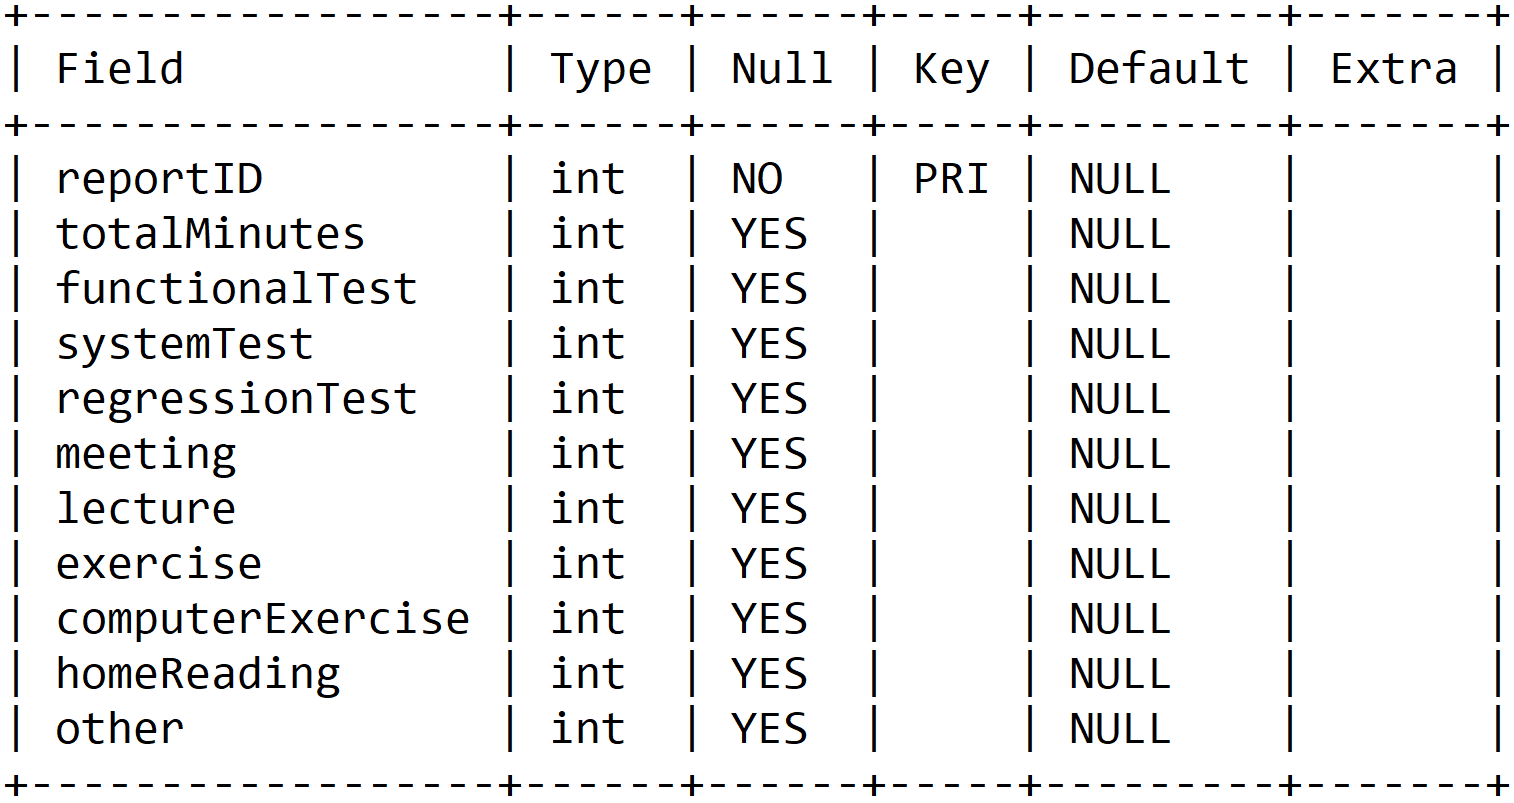
\includegraphics[width=11cm]{images/SQL_tables/activityreport.png}
     \renewcommand\figurename{Figure}
     \caption{A view of the ActivityReport relation and its attributes.}
     \label{fig:my_label}
 \end{figure}
\newline

An ActivityReport table can be created using the following MySQL command:
\newline

\small
\texttt{
\noindent mysql> CREATE TABLE ActivityReport (\newline
\indent\indent\indent -> reportID Integer NOT NULL,\newline
\indent\indent\indent -> totalMinutes Integer,\newline
\indent\indent\indent -> functionalTest Integer,\newline
\indent\indent\indent -> systemTest Integer,\newline
\indent\indent\indent -> regressionTest Integer,\newline
\indent\indent\indent -> meeting Integer,\newline
\indent\indent\indent -> lecture Integer,\newline
\indent\indent\indent -> exercise Integer,\newline
\indent\indent\indent -> computerExercise Integer,\newline
\indent\indent\indent -> homeReading Integer,\newline
\indent\indent\indent -> other Integer,\newline
\indent\indent\indent -> PRIMARY KEY(reportID),\newline
\indent\indent\indent -> FOREIGN KEY(reportID) REFERENCES TimeReport(reportID)\newline
\indent\indent\indent -> ON UPDATE CASCADE ON DELETE CASCADE\newline
\indent\indent\indent -> );\newline
}
\normalsize


\subsection{DocumentTimeD/I/F/R Relation}
As mentioned earlier, there are four different activity types in the time documentation: \emph{Development and documentation (D)}, \emph{Informal review (I)}, \emph{Formal review (F)} and \emph{Rework, improvement or correction (R)}. All of these relations contain the same attributes mainly concerning the various documents. Besides these attributes, there is one attribute concerning the totalMinutes. The purpose of this attribute is to oversee the amount of minutes spent on each activity type. Since each document continuously is in a different stage, it was concluded to include different phases as activity types to ensure that the time reports are comprehensible. All of these tables can be created by using the same SQL statement. The appearance of each of these tables can be viewed in Figure 5.

\begin{figure}[H]
     \centering
     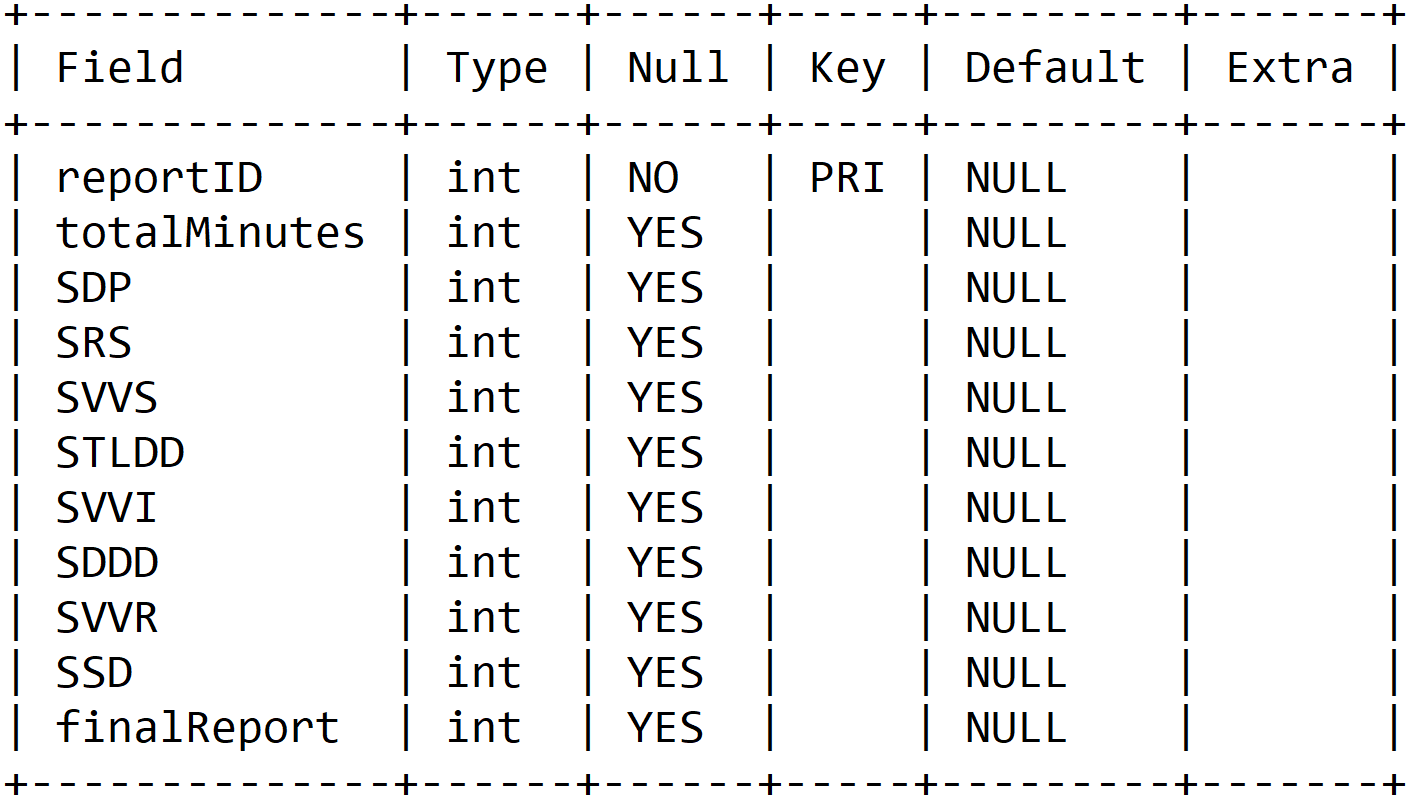
\includegraphics[width=11cm]{images/SQL_tables/documenttime.png}
     \renewcommand\figurename{Figure}
     \caption{A view of a DocumentTime relation and its attributes.}
     \label{fig:my_label}
 \end{figure}
\newline

A DocumentTime table can be created using the following MySQL command:
\newline

\small
\texttt{
\noindent mysql> CREATE TABLE TimeDevelopments (\newline
\indent\indent\indent -> reportID Integer NOT NULL,\newline
\indent\indent\indent -> totalMinutes Integer,\newline
\indent\indent\indent -> SDP Integer,\newline
\indent\indent\indent -> SRS Integer,\newline
\indent\indent\indent -> SVVS Integer,\newline
\indent\indent\indent -> STLDD Integer,\newline
\indent\indent\indent -> SVVI Integer,\newline
\indent\indent\indent -> SDDD Integer,\newline
\indent\indent\indent -> SVVR Integer,\newline
\indent\indent\indent -> SSD Integer,\newline
\indent\indent\indent -> finalReport Integer,\newline
\indent\indent\indent -> PRIMARY KEY(reportID),\newline
\indent\indent\indent -> FOREIGN KEY(reportID) REFERENCES TimeReport(reportID)\newline
\indent\indent\indent -> ON UPDATE CASCADE ON DELETE CASCADE );\newline
}
\normalsize
\newpage
\section{Description of Classes}
This section describes all classes and their public methods.

\subsection{Database}
\subsubsection{addUser()}
Adds a user to the database.
\subsubsection{removeUser()}
Removes a user and all related time reports from the database.
\subsubsection{retrieveTimereports()}
Retrieves a list of all time reports from the database.
\subsubsection{viewTimereport()}
Retrieves a specific time report from the database.
\subsubsection{signTimereports()}
Changes all timereports according to user input.
\subsubsection{viewUsers()}
Retrieves a list of all users from the database.
\subsubsection{setProjectLeader()}
Changes a users role to project leader [1] in the database.
\subsubsection{newTimereport()}
Adds a new time report to the database.
\subsubsection{updateTimereport()}
Changes an existing unsigned time report according to user input.
\subsubsection{deleteTimereport()}
Removes an unsigned time report from the database. 

\subsubsection{getSummary()}
Retrieves a summary of all reported time.
\subsubsection{updateRole()}
Changes a users role according to user input. Cannot change a users role to PG [1].
\subsubsection{checkLogin()}
Checks if the login credentials are correct.
\subsubsection{getPassword()}
Retrieves the users current password.
\subsubsection{setPassword()}
Checks if the new password is valid by using getPassword(). If it's valid, it replaces the old password. If not, the password remains unchanged.
\subsubsection{getEmail()}
Retrieves the users email.

\subsection{UserBean}
\subsubsection{populateBean()}
Sets all attributes in the bean according to user input.
\subsubsection{getUserName()}
Gets the username contained in the bean.
\subsubsection{getEmail()}
Gets the email contained in the bean.
\subsubsection{getRole()}
Gets the role contained in the bean.

\subsection{UserManagementBean}
\subsubsection{populateBean()}
Sets all attributes in the bean according to the database.
\subsubsection{getUserName()}
Gets the username contained in the bean.
\subsubsection{getUserList()}
Gets the userlist contained in the bean.
\subsubsection{getRole()}
Gets the role contained in the bean.
\subsection{TimeReportBean}
\subsubsection{populateBean()}
Sets all attributes in the bean according to user input.
\subsubsection{getUsername()}
Gets the username contained in the bean.
\subsubsection{getWeek()}
Gets the week of the time report contained in the bean.
\subsubsection{getReportValues()}
Gets the values of the time report contained in the bean.

\subsection{TimeReportManagementBean}
\subsubsection{populateBean()}
Sets all attributes in the bean according to user input.
\subsubsection{timeReportList()}
Gets a list of all time reports contained in the bean.
\subsubsection{getUserName()}
Gets the username contained in the bean.

\subsection{PasswordHandler}
\subsubsection{hashPassword()}
Returns the hash of a given password.
\subsubsection{generatePassword()}
Randomly generates a new password for a user.
\subsection{MailHandler}
\subsubsection{sendPasswordMail()}
Sends an email containing a password generated from PasswordHandler.


\section{Class Diagram}

\begin{figure}[H]
    \centering
    \includegraphics[scale=0.5]{images/ClassDiagram.png}
    \caption{Diagram containing an overview of all classes.}
    \label{fig:classDiagram}
\end{figure}


\section{Sequence Diagrams}
\subsection{LoginServlet}

\begin{figure}[H]
    \centering
    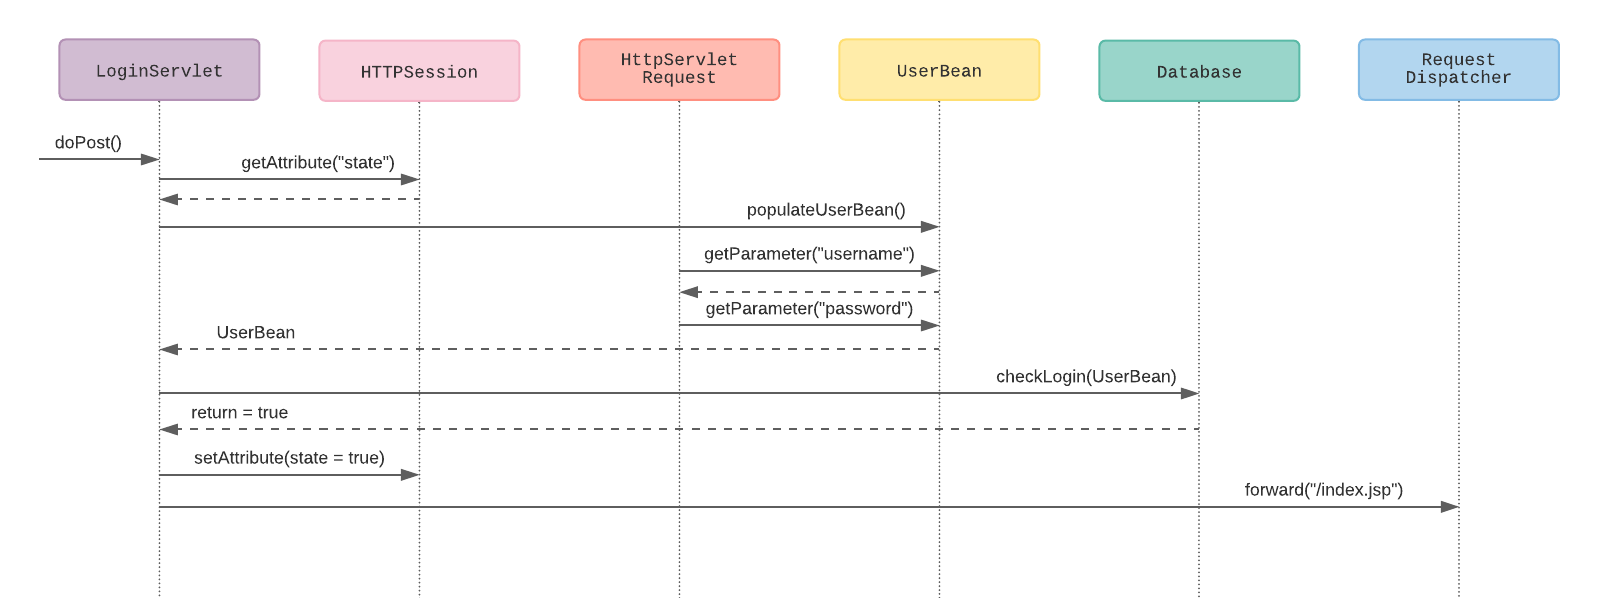
\includegraphics[scale=0.6]{images/successfulLogin.png}
    \caption{Sequence diagram for a successful login.}
    \label{fig:successfulLogin}
\end{figure}

\begin{figure}[H]
    \centering
    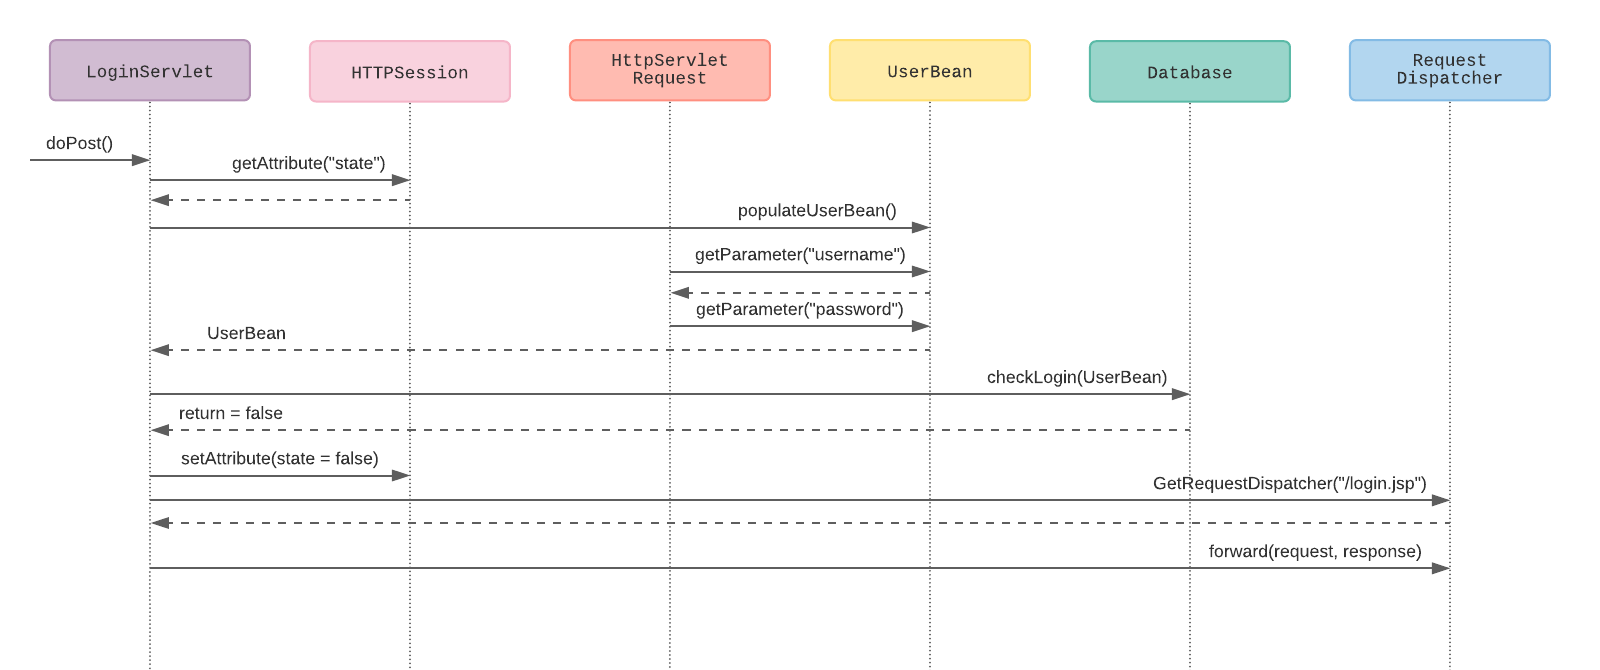
\includegraphics[scale=0.6]{images/failedLogin.png}
    \caption{Sequence diagram for a failed attempt to login.}
    \label{fig:failedLoginAttempt}
\end{figure}

\pagebreak
\subsection{UserManagementServlet}

\begin{figure}[H]
    \centering
    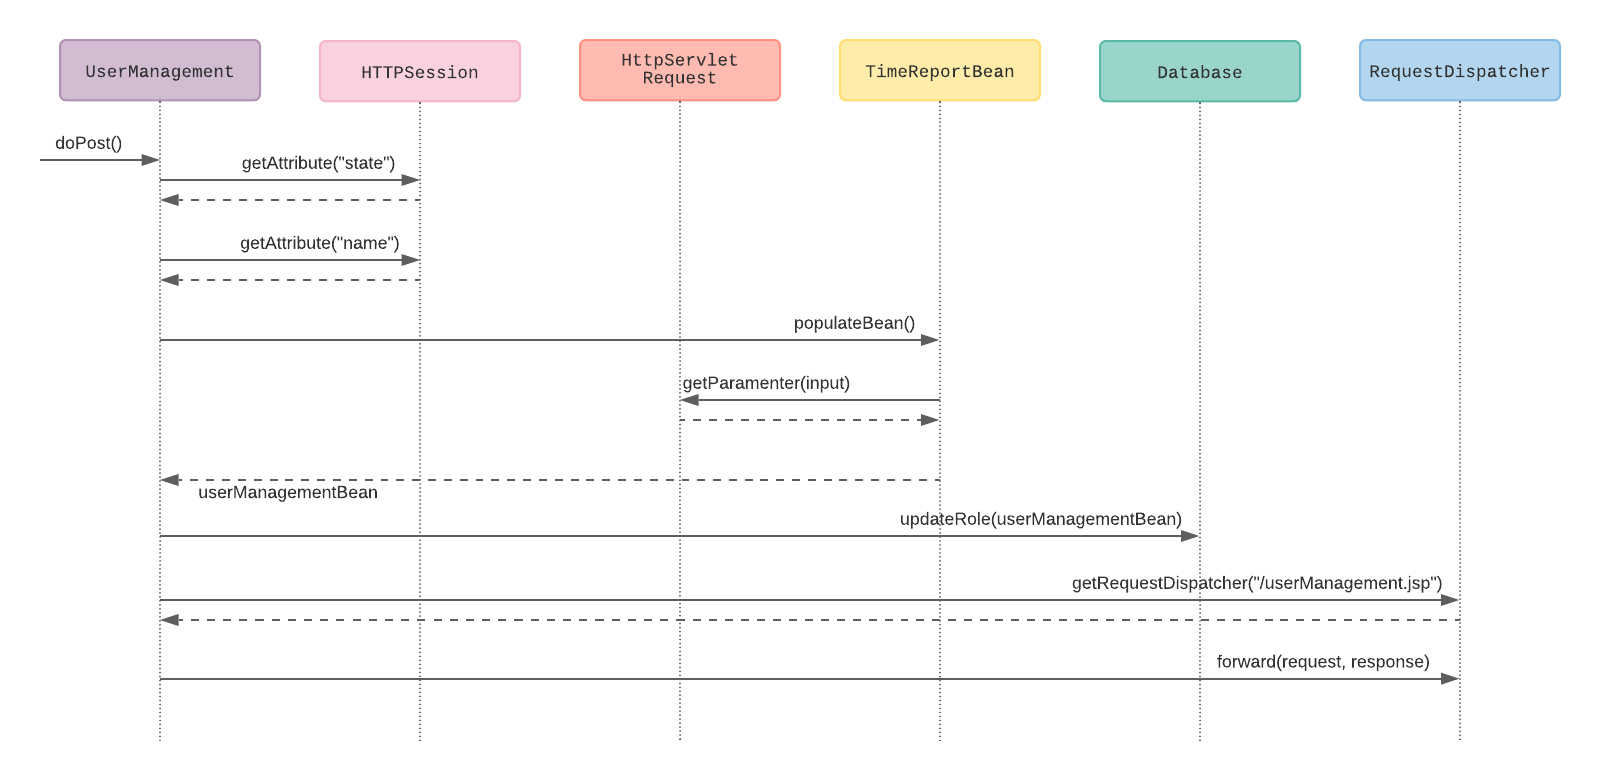
\includegraphics[scale=0.6]{images/updateRole.png}
    \caption{Sequence diagram for the process of updating the role of a project member.}
    \label{fig:successfulLogin}
\end{figure}

\begin{figure}[H]
    \centering
    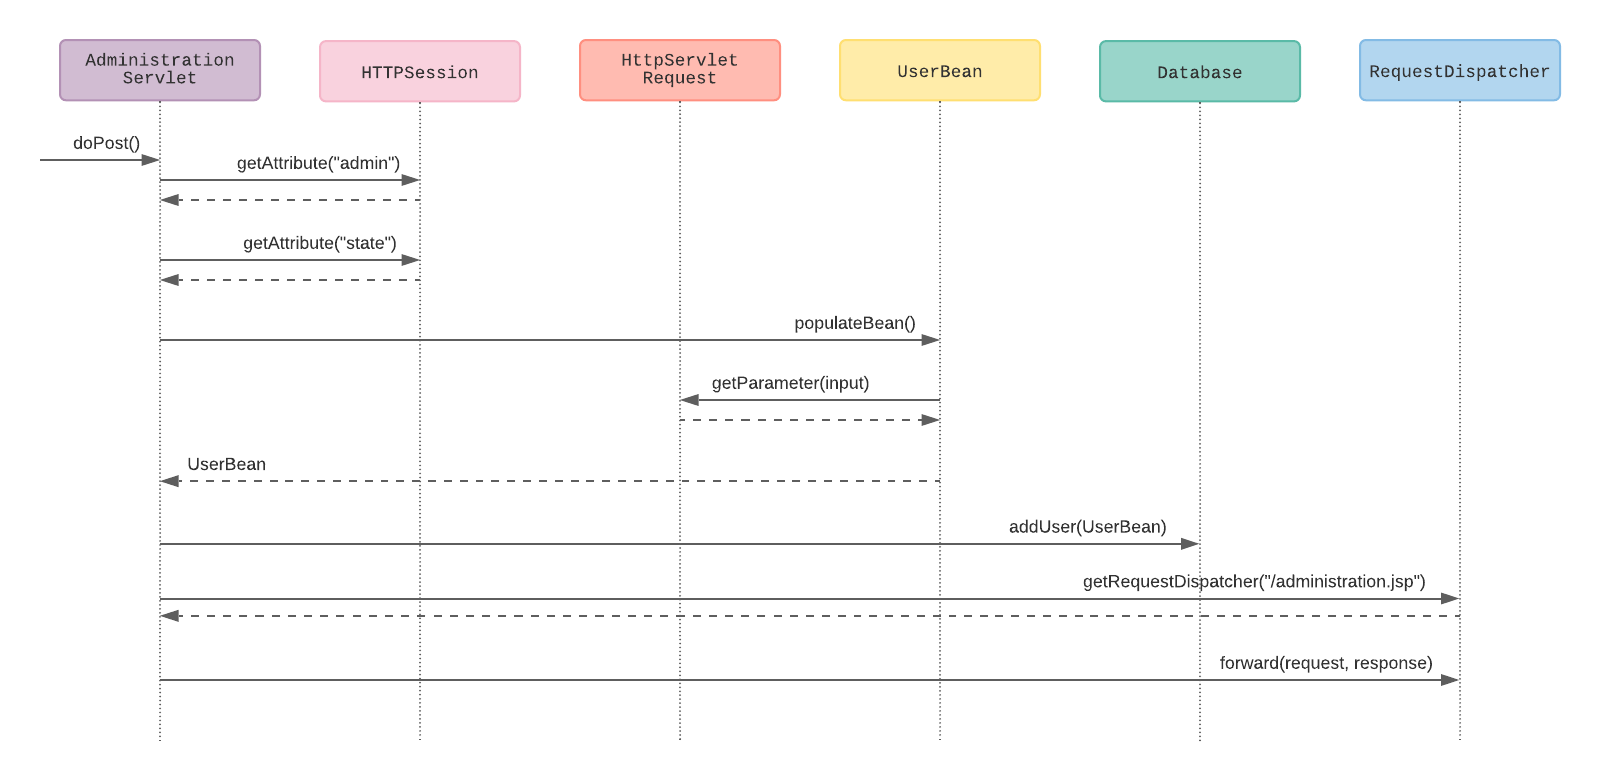
\includegraphics[scale=0.6]{images/addUser.png}
    \caption{Sequence diagram for adding a user by administrator.}
    \label{fig:failedLoginAttempt}
\end{figure}

\pagebreak
\subsection{PasswordChangerServlet}

\begin{figure}[h]
    \centering
    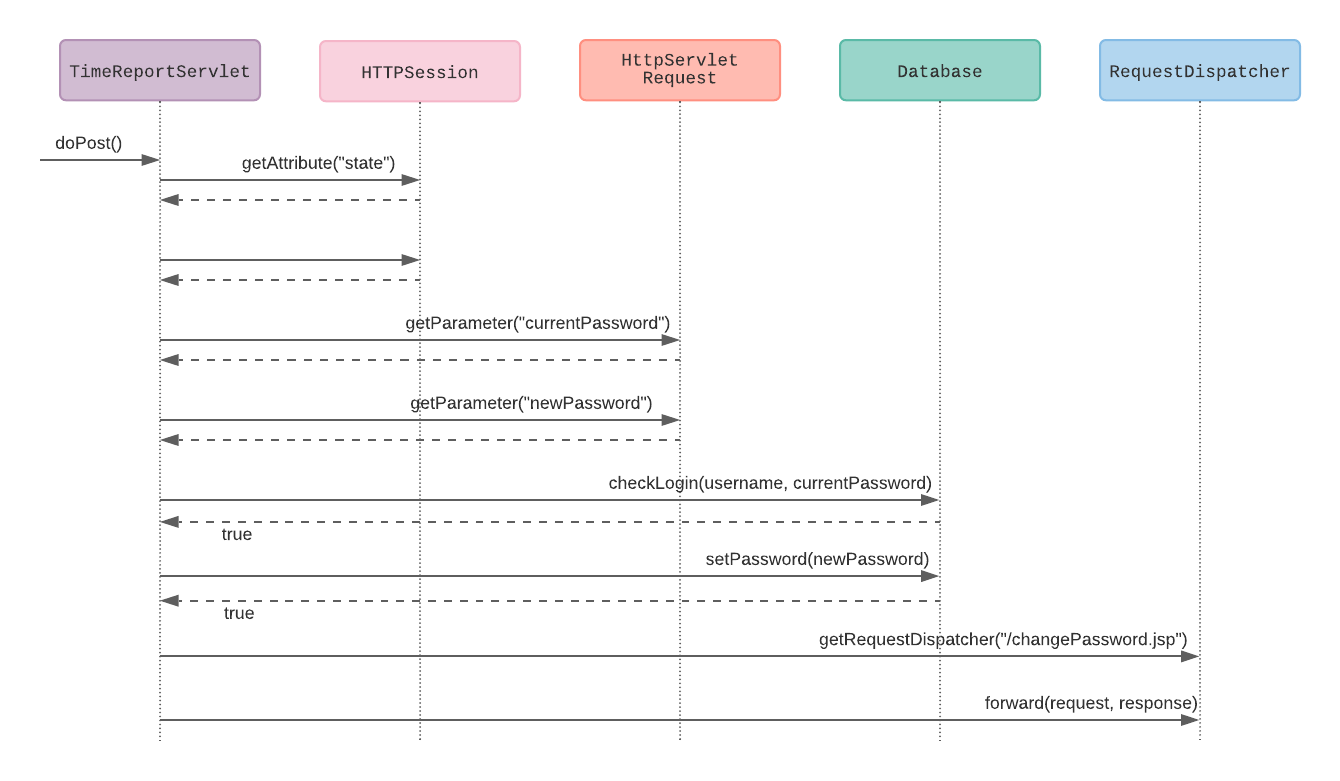
\includegraphics[scale=0.6]{images/successfulPasswordChange.png}
    \caption{Sequence diagram for a successful password change.}
    \label{fig:sucessfulPasswordChange}
\end{figure}

\begin{figure}[H]
    \centering
    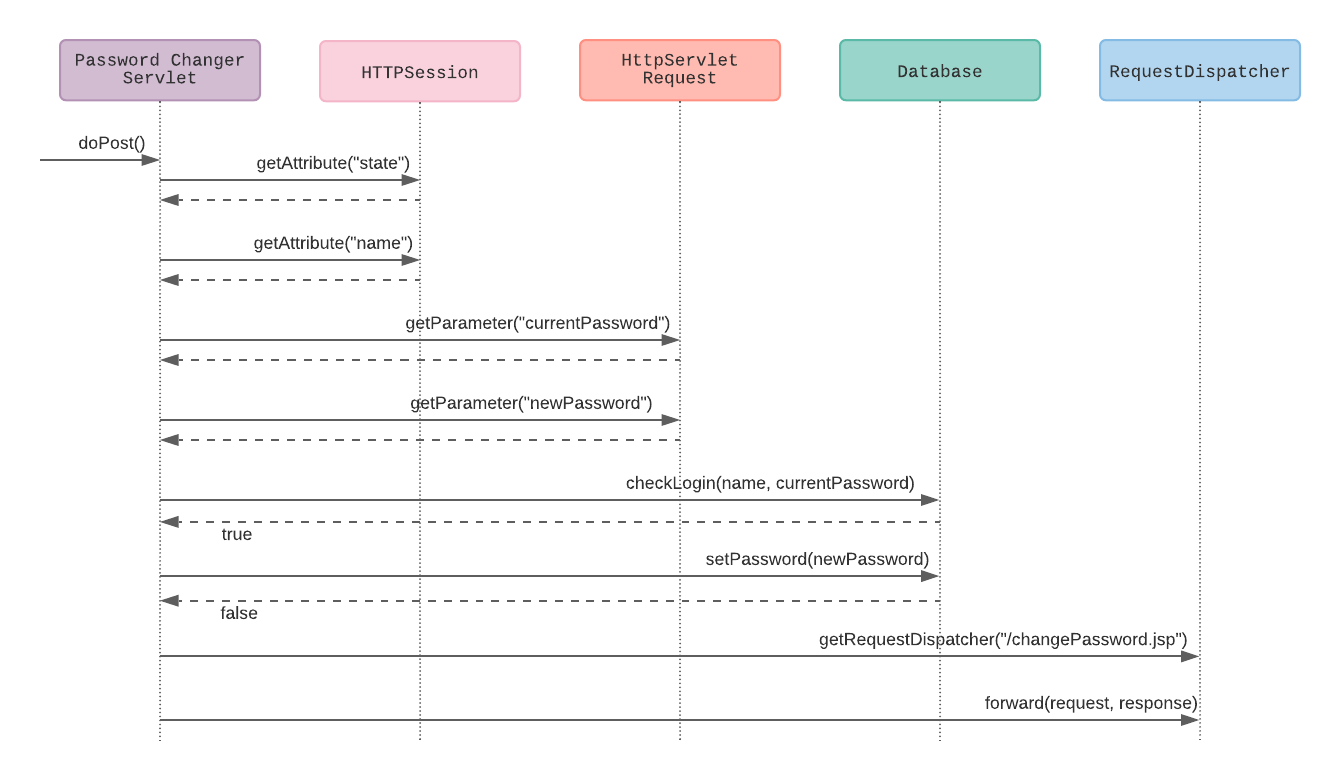
\includegraphics[scale=0.6]{images/unsuccessfulPasswordChange.png}
    \caption{Sequence diagram for a failed attempt to change password.}
    \label{fig:failedPasswordChange}
\end{figure}

\begin{figure}[H]
    \centering
    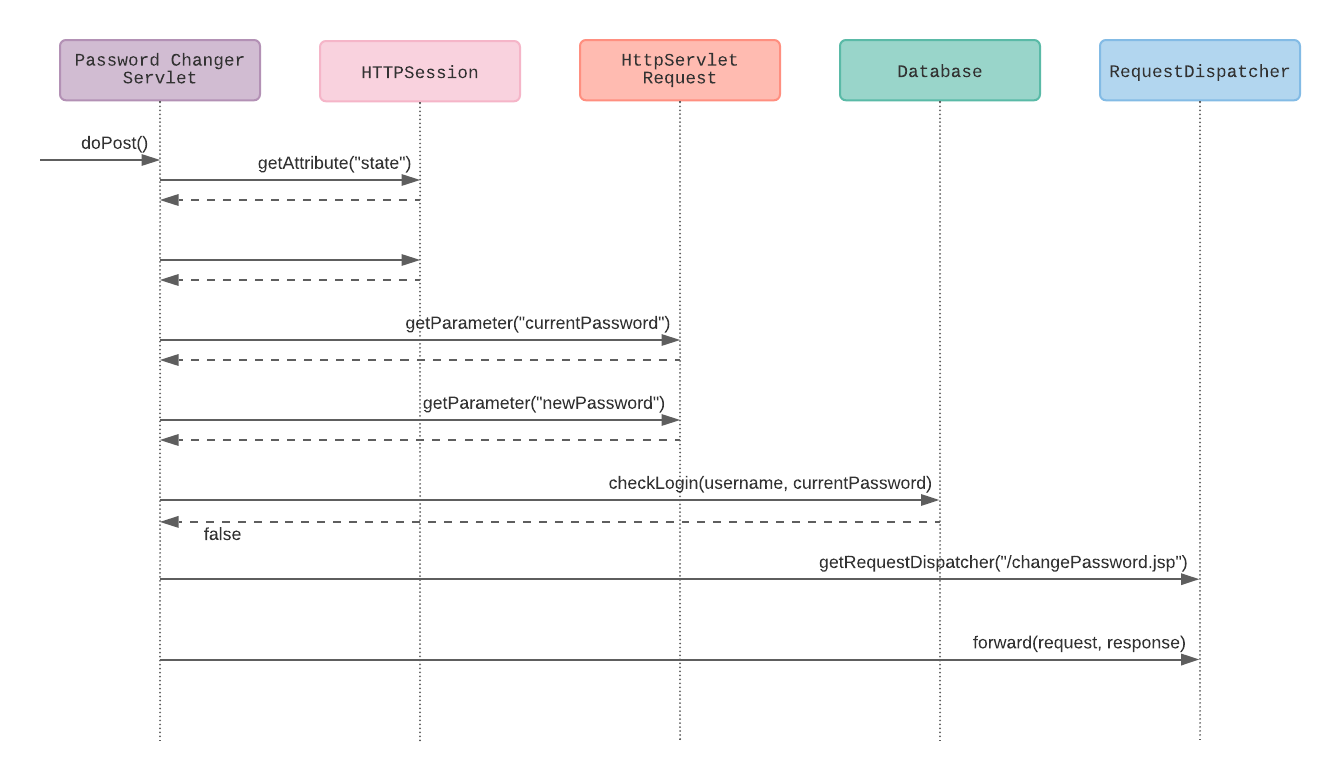
\includegraphics[scale=0.6]{images/changePasswordFalseInput.png}
    \caption{Sequence diagram for a failed attempt to change password due to incorrect user input.}
    \label{fig:failedPasswordChangeIncorrectInput}
\end{figure}

\pagebreak

\subsection{TimeReportServlet}

\begin{figure}[H]
    \centering
    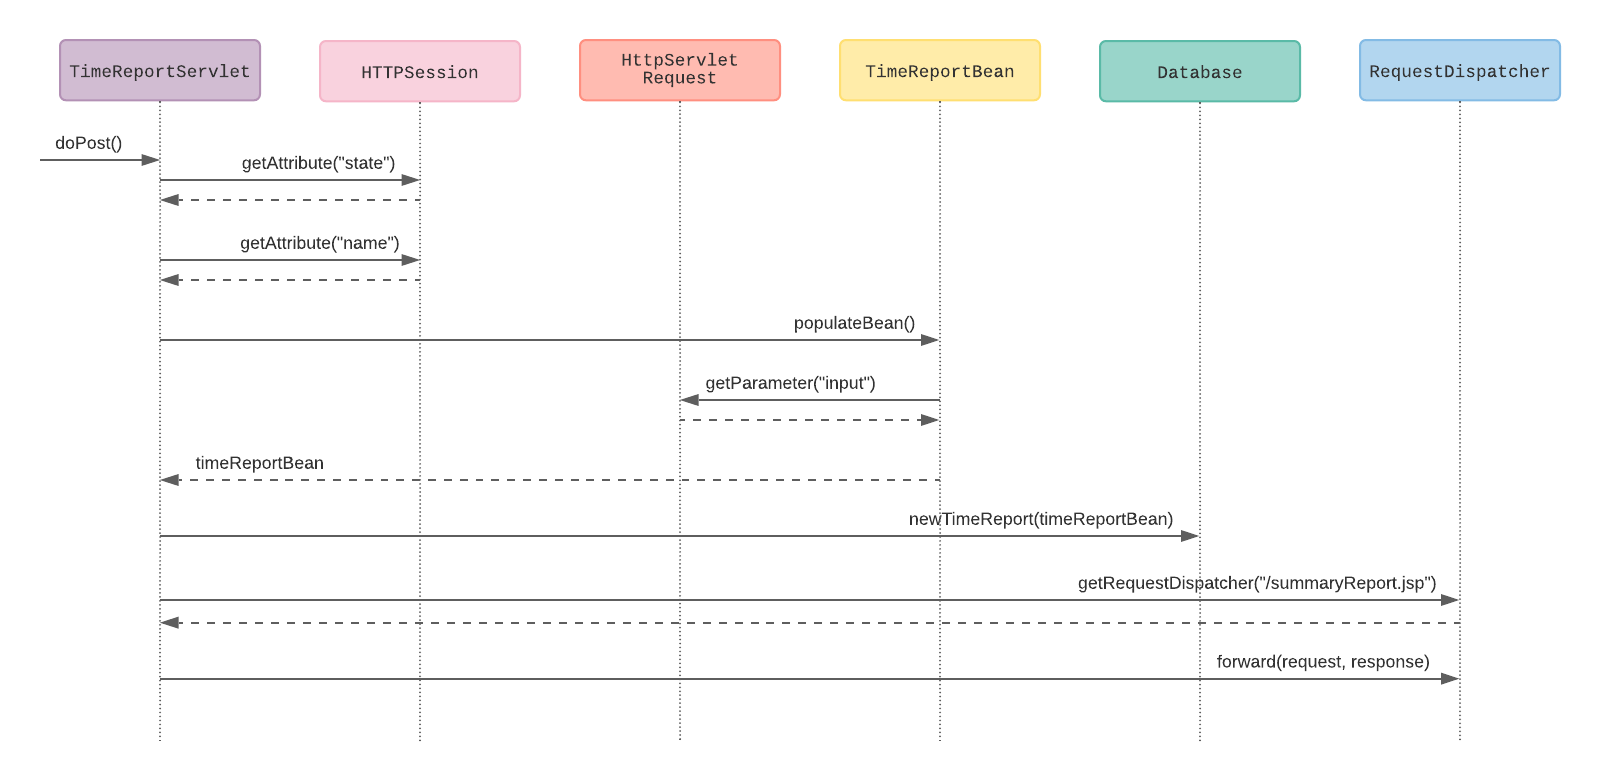
\includegraphics[scale=0.6]{images/newTimeReport.png}
    \caption{Sequence diagram for adding a new Time Report.}
    \label{fig:newTimeReport}
\end{figure}

\begin{figure}[H]
    \centering
    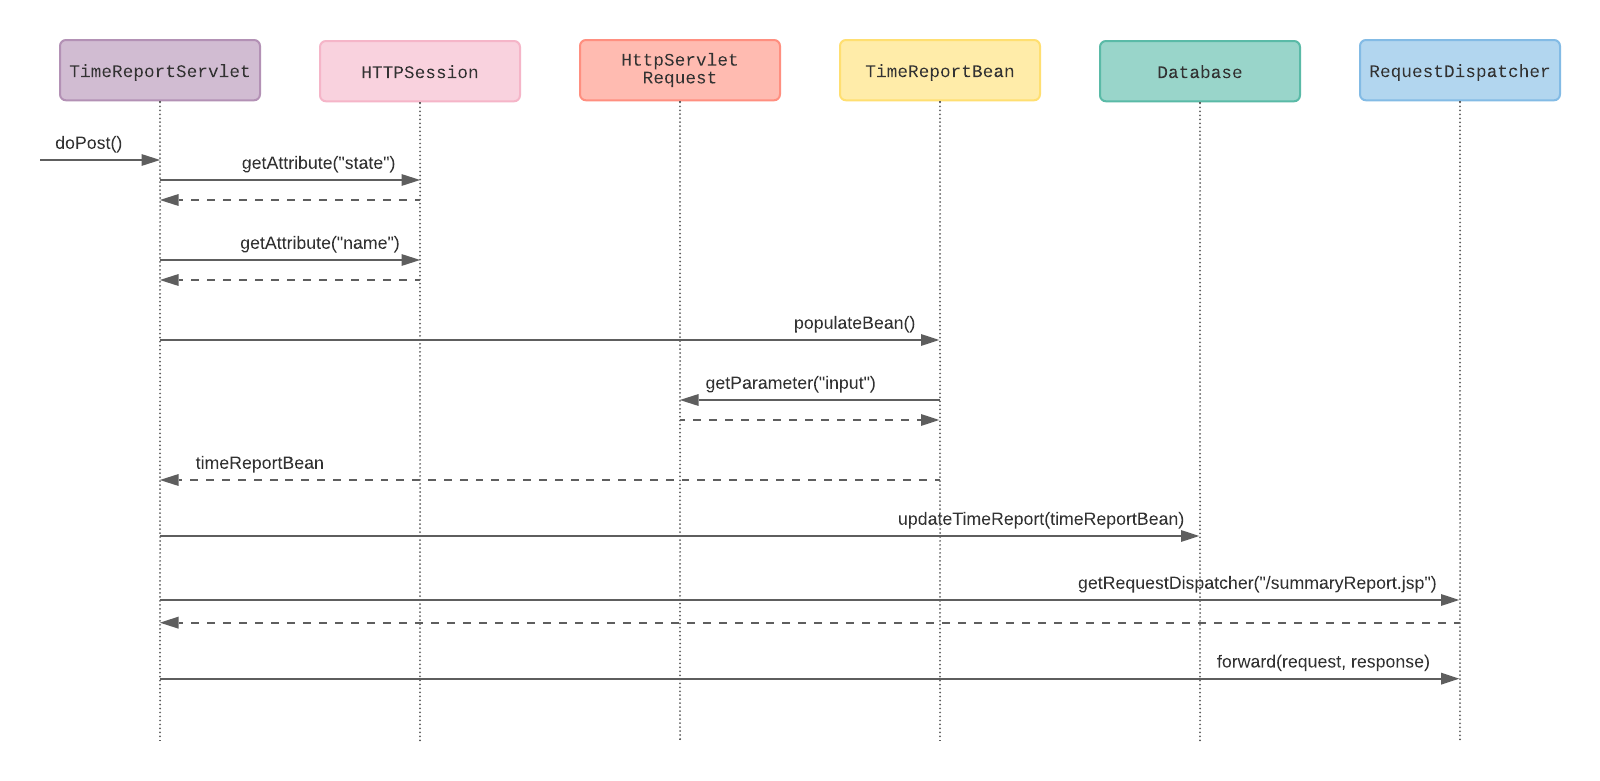
\includegraphics[scale=0.6]{images/editTimeReport.png}
    \caption{Sequence diagram for a editing a Time Report.}
    \label{fig:editTimeReport}
\end{figure}

\subsection{TimeReportManagementServlet}

\begin{figure}[H]
    \centering
    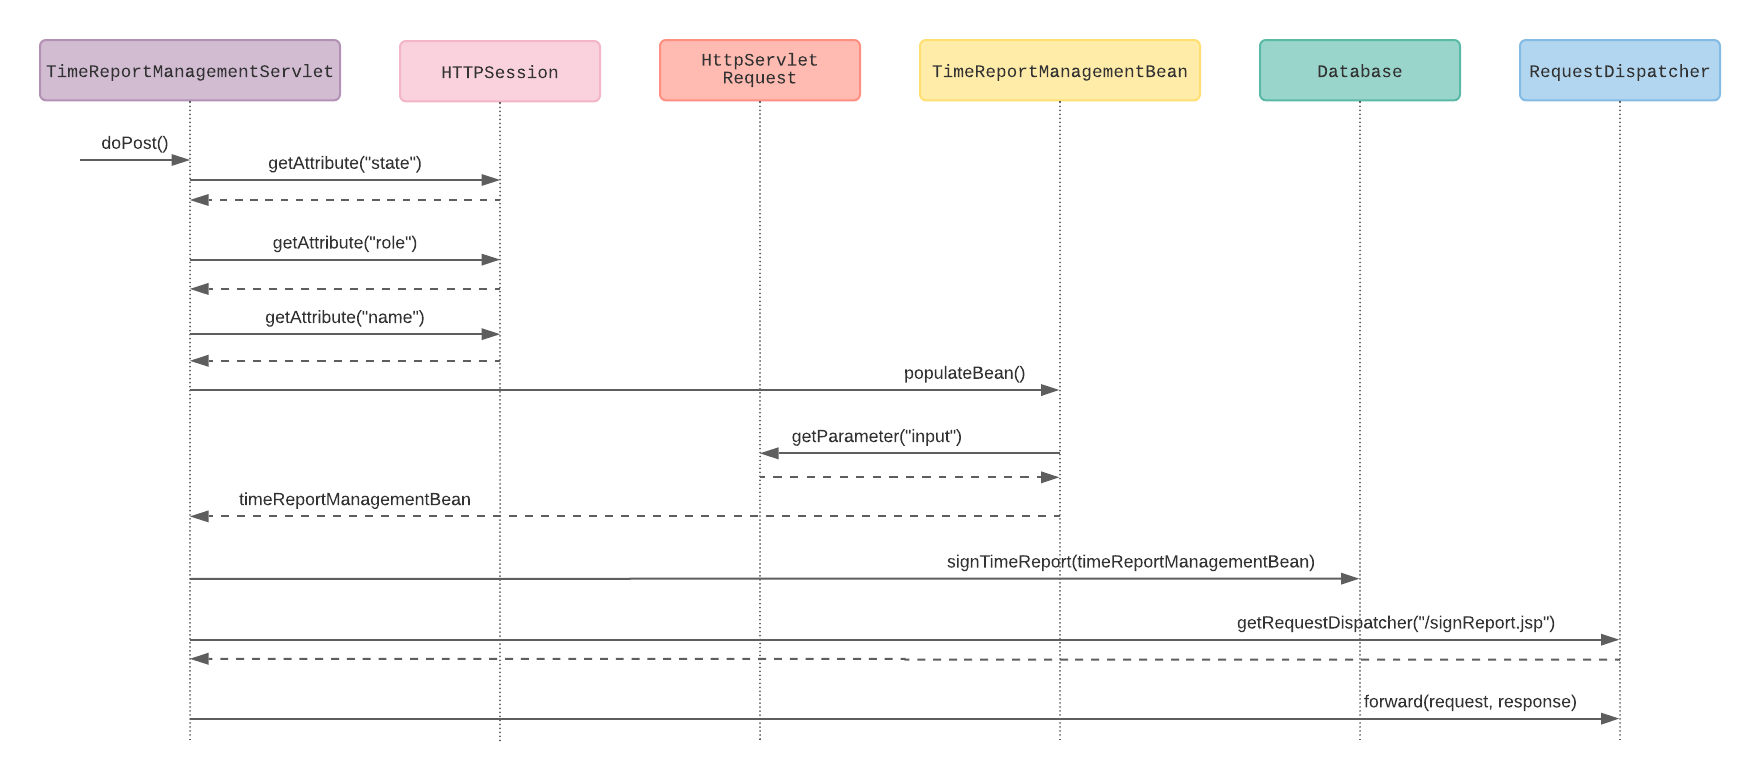
\includegraphics[scale=0.6]{images/signUnsignReports.png}
    \caption{Signing/unsigning a Time Report. This can only be done by the project leader.}
    \label{fig:signunsign}
\end{figure}



%---------Document ends here-----------

\end{document}
